\documentclass{article}

\PassOptionsToPackage{numbers, sort, compress}{natbib}
\usepackage[main,final]{neurips_2025}

\usepackage{iftex}
\ifPDFTeX
    \usepackage[T2A]{fontenc}
    \usepackage[utf8]{inputenc}
\else
    \usepackage{fontspec}
    \setmainfont{Times New Roman}
    \setsansfont{Arial}
    \setmonofont{Courier New}
\fi
\usepackage[english,russian]{babel}
\usepackage{hyperref}
\usepackage{url}
\usepackage{booktabs}
\usepackage{nicefrac}
\usepackage{microtype}
\usepackage{xcolor}
\usepackage{graphicx}
\usepackage{amsmath,amssymb,amsfonts}

\graphicspath{{../slides/figs/}}

\title{Сравнение стратегий разбиения патентных документов\\для семантического поиска и RAG}

\author{
  Елизавета Кожемякова\\
  TODO: организация\\
  \texttt{TODO: email}\\
  \And
  Роман Ищенко\\
  TODO: организация\\
  \texttt{TODO: email}\\
}

\begin{document}

\maketitle

\begin{abstract}
Качество семантического поиска и генерации с использованием извлеченной информации (Retrieval-Augmented Generation, или RAG) по длинным техническим документам во многом определяется тем, каким образом документ разбивается на фрагменты («чанки») перед векторизацией. Данная работа посвящена поиску схемы разбиения и векторизации патентных документов, которая повышает качество поиска при использовании готовых моделей векторных представлений текста без их дообучения. Патент~--- длинный и неоднородный документ. Его разделы~--- сущность изобретения, уровень техники, подробное описание, формула~--- существенно различаются по информативности, а разбиение на фрагменты фиксированной длины смешивает их, размывает смысловой сигнал и позволяет шаблонным формулировкам доминировать в выдаче. Предлагается формировать фрагменты по смысловой структуре самого документа~--- по разделам и по блокам, выделяемым триггерными фразами,~--- а не по длине текста. Структурно-ориентированные схемы сравниваются на корпусе из 37\,727 патентов с разбиением фиксированной длины, группировкой абзацев и иерархическим индексированием на основе суммаризации языковой моделью. Кроме того, для каждого раздела оценивается его вклад в качество поиска.
Полученные результаты позволяют определить, какие части патентного документа следует векторизовать в первую очередь. Практическая ценность работы состоит в рекомендациях по выбору схемы разбиения для поиска, кластеризации и RAG по научно-технической информации.
\end{abstract}

\textbf{Ключевые слова:} генерация с использованием извлеченной информации, плотный поиск, разбиение документов, патентные документы, векторные представления текста

%%%%%%%%%%%%%%%%%%%%%%%%%%%%%%%%%%%%%%%%%%%%%%%%%%%%%%%%%%%%
\section{Введение}\label{sec:intro}

Патентные документы~--- один из основных источников научно-технической информации~\citep{jiang2025patentsurvey}. Поиск по ним необходим при проверке новизны изобретения и при анализе состояния области. Все чаще такой поиск ведется по смыслу, а не по ключевым словам, с помощью векторных представлений текста~\citep{reimers2019sbert,karpukhin2020dpr} и генерации с использованием извлеченной информации (RAG)~\citep{lewis2020rag}, при которой языковая модель отвечает на вопрос по найденным фрагментам. Эксперту и модели доступно только то, что попало в выдачу, поэтому качество результата во многом определяется тем, как патент разбит на фрагменты перед векторизацией. Этому этапу и посвящена работа.

\emph{Разбиением} (chunking) называется деление документа на фрагменты, каждый из которых модель векторных представлений переводит в вектор независимо от остальных. При \emph{векторном поиске} фрагменты ранжируются по близости их векторов к вектору запроса. Патент имеет устойчивую структуру: реферат, описание уровня техники, сущность изобретения, подробное описание и формула изобретения. \emph{Уровень техники}~--- совокупность сведений, ставших общедоступными до даты приоритета заявки.

Длина патента обычно превышает входное окно модели векторных представлений. Передача полного текста языковой модели проблему не решает: сведения из середины длинного контекста модель использует хуже, чем из его начала и конца~\citep{liu2024lost}. Поэтому патент разбивают на фрагменты, как правило фиксированной длины. При таком разбиении в один фрагмент попадают части разных разделов, например окончание описания уровня техники и начало сущности изобретения. Кроме того, стандартные патентные формулировки, повторяющиеся в тысячах документов, повышают сходство патентов, не связанных по содержанию. Открытым остается вопрос, какие разделы патента следует векторизовать и с какой гранулярностью.

Разбиение по естественным границам текста, в частности группировка абзацев, заметно превосходит разбиение фиксированной длины~\citep{shaukat2026chunking}, однако все абзацы в ней считаются равноценными, а на патентах она не проверялась. RAPTOR~\citep{sarthi2024raptor} улучшает поиск за счет дерева кратких содержаний над фрагментами, но требует языковой модели при индексации. Ближе всего к настоящей работе разбиение по элементам документа~\citep{jimenoyepes2024financial}: оно использует структуру документа, но определяет ее по внешней разметке, а не по смысловой роли фрагментов. Ни один из этих подходов не учитывает различия в роли разделов патента.

В работе предложен способ разбиения патентов для векторного поиска и RAG, направленный на повышение качества поиска при неизменной модели векторных представлений. Его отличие от известных подходов состоит в том, что фрагменты выделяются по смысловой структуре патента: по разделам и по блокам, которые открываются характерными для патентов формулировками. Поскольку разделы векторизуются раздельно, становится возможным оценить вклад каждого из них в качество поиска.

Для этого решаются следующие задачи: выделить в тексте патента смысловые разделы и блоки, построить на их основе схемы разбиения, сравнить эти схемы с базовыми методами и оценить вклад отдельных разделов в качество поиска.

\textbf{Вклад работы.}
\begin{itemize}
    \item Схемы структурного разбиения патентов по разделам и по блокам с характерными фразами, которые работают с готовыми моделями векторных представлений.
    \item Сравнение этих схем с разбиением по длине, группировкой абзацев и RAPTOR в одинаковых условиях.
    \item Оценка того, какие разделы патента сильнее всего влияют на качество поиска.
    \item Рекомендации по выбору схемы разбиения патентов для поиска и RAG.
\end{itemize}

\textbf{Структура статьи.} В разделе~\ref{sec:rw} приведен обзор литературы, в разделе~\ref{sec:prelim}~--- постановка задачи, в разделе~\ref{sec:method}~--- предлагаемый метод, в разделе~\ref{sec:exp}~--- вычислительный эксперимент. Разделы~\ref{sec:disc} и~\ref{sec:concl} содержат обсуждение результатов и заключение.

\section{Обзор литературы}\label{sec:rw}

Поиск по длинным документам начинается с того, что документ разбивают на фрагменты, и от этого шага зависит, что поисковик вообще сможет найти. Работы на эту тему можно разделить на три группы: одни меняют правила разбиения, другие строят над фрагментами иерархию, третьи обучают модель векторных представлений под конкретную предметную область.

\begin{table}[t]
    \centering
    \small
    \caption{Сравнение подходов к представлению длинных документов для поиска. Дешевые способы разбиения не различают смысловую роль фрагментов, а более сложные требуют языковой модели при индексации или обучения. Структурное разбиение патента занимает свободное место между ними.}
    \label{tab:rw}
    \begin{tabular}{p{0.24\linewidth}p{0.34\linewidth}p{0.34\linewidth}}
        \toprule
        Метод & Сильные стороны & Слабые стороны \\
        \midrule
        Фиксированная длина~\citep{shaukat2026chunking} & Простота, предсказуемый размер индекса & Режет текст посреди мысли, оптимальная длина зависит от данных~\citep{bhat2025chunksize} \\
        Семантическое разбиение~\citep{qu2025semantic} & Границы по смене смысла соседних предложений & Дороже фиксированного разбиения, а на реальных данных его не превосходит \\
        Группировка абзацев~\citep{shaukat2026chunking} & Лучшее качество среди дешевых методов, в том числе на юридических текстах & Абзацы считаются равноценными, нужна разметка абзацев, которой в патентах почти нет \\
        Разбиение по элементам документа~\citep{jimenoyepes2024financial} & Использует структуру документа, заметно улучшает RAG & Структура берется из внешней разметки, а не из смысловой роли фрагментов, на патентах не проверялось \\
        Позднее разбиение~\citep{gunther2024late} & Фрагмент сохраняет контекст всего документа & Требует модели с длинным контекстом \\
        RAPTOR~\citep{sarthi2024raptor} & Поиск на нескольких уровнях подробности, улучшает любой из проверенных поисковиков & Много вызовов LLM при индексации, около 4\% узлов с галлюцинациями, иерархия восстанавливается кластеризацией \\
        PAI-NET~\citep{lee2025painet}, PaECTER~\citep{ghosh2024paecter} & Учитывают специфику патентов, обучены на ссылках экспертов & Требуют обучения модели и не отвечают на вопрос, какие части патента векторизовать \\
        \midrule
        Структурное разбиение (настоящая работа) & Учитывает смысловую роль разделов патента, работает с готовой моделью без LLM и обучения, позволяет оценить вклад каждого раздела & Правила выделения разделов и триггерных фраз зависят от типа документов \\
        \bottomrule
    \end{tabular}
\end{table}

\textbf{Способы разбиения.}
Чаще всего документ разбивают на фрагменты фиксированной длины, обычно от 100 до 512 токенов, и длину выбирают под ограничения модели, а не под устройство текста~\citep{shaukat2026chunking}. Авторы этой работы сравнили 36 стратегий разбиения на шести предметных областях и пяти моделях, не меняя поисковик. Лучше всего сработала простая группировка абзацев (Paragraph Group Chunking: по два абзаца с перекрытием в один): nDCG@5 у нее 0,459, у разбиения фиксированной длины~--- 0,244. Более сложное семантическое разбиение такого прироста не дало. К похожему выводу пришли и в работе~\citep{qu2025semantic}: разбиение по близости векторов предложений обходится заметно дороже, а на реальных данных не обгоняет разбиение фиксированной длины. При этом и у фиксированного разбиения нет универсального размера: оптимальная длина фрагмента зависит от набора данных и модели~\citep{bhat2025chunksize}, поэтому этот базовый метод нужно проверять при нескольких длинах.

Ближе всего к нашей идее работа~\citep{jimenoyepes2024financial}, где финансовые отчеты разбивают по элементам документа~--- заголовкам, абзацам, таблицам,~--- и это заметно улучшает RAG. Элементы там, однако, выделяются по внешней разметке, а не по смысловой роли фрагмента. Патентов нет ни в одной из перечисленных работ. В группировке абзацев к тому же все абзацы считаются равноценными, независимо от того, о чем они. Для нашего корпуса есть и практическое препятствие: в текстах патентов почти нет разметки абзацев, поэтому группировка абзацев на нем неприменима в исходном виде.

Отдельно стоит позднее разбиение (late chunking)~\citep{gunther2024late}. Границы фрагментов в ней прежние, меняется способ получить их векторы: документ целиком проходит через модель с длинным контекстом, и векторы токенов усредняются уже внутри каждого фрагмента. Так фрагмент сохраняет контекст соседей, но для этого нужна модель с длинным окном, поэтому в число базовых методов позднее разбиение не включено.

\textbf{Иерархические представления.}
RAPTOR~\citep{sarthi2024raptor} ищет сразу на нескольких уровнях подробности. Фрагменты кластеризуются, большая языковая модель пишет краткое содержание каждого кластера, и процедура повторяется, пока не получится дерево. Поиск идет по всем его узлам одновременно. На общие вопросы отвечают верхние узлы, на вопросы о деталях~--- исходные фрагменты. Со всеми тремя поисковиками, с которыми метод проверяли (SBERT, DPR и BM25), качество выросло.

Цена этого~--- обращения к языковой модели при индексации, которые на корпусе из десятков тысяч патентов обходятся дорого. Около 4\% порожденных узлов содержат галлюцинации. Кроме того, иерархию RAPTOR получает кластеризацией, хотя у патента она уже есть в готовом виде.

\textbf{Модели для патентов.}
PAI-NET~\citep{lee2025painet} решает задачу со стороны модели. Кодировщик обучают на тройках: патент, документ уровня техники, на который он ссылается, и не связанный с ним патент того же класса. Среднее значение обратного ранга (MRR) вырастает до 0,76 против 0,56--0,59 у универсальных моделей. На ссылках экспертов обучена и открытая модель PaECTER~\citep{ghosh2024paecter}, которая в предсказании цитирований превосходит как BERT for Patents, так и универсальные модели. Еще раньше в работе~\citep{helmers2019prior} ссылки из отчетов о поиске использовали как эталон при оценке поиска уровня техники по полному тексту. Для настоящей работы важна общая для этих работ идея: ссылки на уровень техники проставляет эксперт, поэтому их можно использовать как оценки релевантности, не размечая данные вручную. Обучение отдельной модели в нашу постановку не входит.

\textbf{Нерешенная задача.}
Из таблицы~\ref{tab:rw} видно, что дешевые способы разбиения не различают смысловую роль фрагментов: уровень техники, формула и описание технического результата для них одинаковы. Подходы, которые учитывают содержание глубже, требуют языковой модели при индексации или обучения модели. В рассмотренных работах не проверялось, какой раздел патента больше всего помогает поиску: формула, сущность изобретения, уровень техники или подробное описание. Нужна схема разбиения, которая опирается на смысловую структуру патента и обходится готовой моделью векторных представлений без вызовов языковой модели. Построить и проверить такую схему~--- цель настоящей работы. Для сравнения взяты разбиение фиксированной длины, группировка абзацев~\citep{shaukat2026chunking} и RAPTOR~\citep{sarthi2024raptor}.

\section{Постановка задачи}\label{sec:prelim}

TODO

\section{Метод}\label{sec:method}

TODO

\section{Вычислительный эксперимент}\label{sec:exp}

\subsection{Выделение разделов поиском по ключевым словам}\label{sec:exp-sections}

Прежде чем разбивать патент по разделам, нужно убедиться, что эти разделы можно найти автоматически. Первый эксперимент проверяет это на корпусе из 37\,727 патентов в области покрытий и заодно показывает, как часто разбиение фиксированной длины смешивает разные разделы в одном фрагменте. Используется текст описания патента. Разметки разделов и абзацев в нем нет, заголовки записаны прописными буквами прямо в тексте.

Описание патента $d$ рассматривается как последовательность разделов $s_1, \ldots, s_K$, где каждый раздел тянется от своего заголовка до следующего. Заголовки ищутся так: в начале предложений выбираются последовательности слов, записанных прописными буквами, и те из них, что встречаются хотя бы в 20 патентах, образуют словарь. Затем по ключевым словам каждому заголовку приписывается один из восьми типов раздела. Так, заголовок со словом BACKGROUND относится к уровню техники, а со словом SUMMARY к сущности изобретения. Для сравнения то же описание разбивается на фрагменты $c_j$ по 10 предложений с перекрытием в одно предложение. Фрагмент, внутри которого проходит граница раздела, будем называть смешанным.

В словарь вошел 291 вариант заголовка. Разделы удалось выделить у 98,5\% патентов, в среднем по 5,15 типа на патент. Среди 1,54~млн фрагментов фиксированной длины смешанными оказались 10,1\%, причем такие фрагменты встречаются у 99,3\% патентов. Длины разделов приведены в таблице~\ref{tab:sections}, пример разбиения показан на рис.~\ref{fig:sections_chunks}.

\begin{table}[t]
    \centering
    \small
    \caption{Разделы описания патента: доля патентов, где раздел найден, доля раздела в описании и длина в предложениях (медиана, в скобках квантили 10\% и 90\%).}
    \label{tab:sections}
    \begin{tabular}{lccc}
        \toprule
        Раздел & Доля патентов & Доля описания & Предложений \\
        \midrule
        Подробное описание & 89\% & 63\% & 180 (61--445) \\
        Примеры & 46\% & 25\% & 78 (22--236) \\
        Сущность изобретения & 86\% & 13\% & 18 (5--62) \\
        Уровень техники & 91\% & 8\% & 16 (6--46) \\
        Чертежи & 75\% & 6\% & 14 (5--57) \\
        Ссылки на связанные заявки & 56\% & 4\% & 7 (4--20) \\
        Область техники & 58\% & 1\% & 2 (2--4) \\
        \bottomrule
    \end{tabular}
\end{table}

\begin{figure}[t]
    \centering
    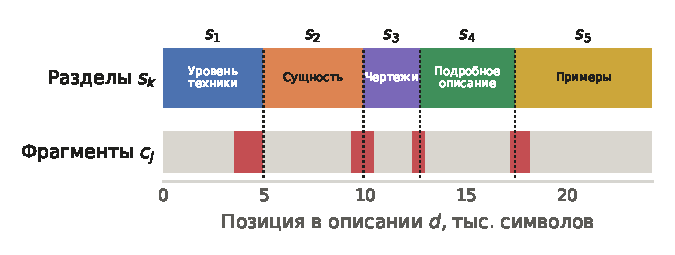
\includegraphics[width=0.85\linewidth]{sections_chunks}
    \caption{Разделы $s_k$ описания патента $d$ и фрагменты $c_j$ базового разбиения. Красные фрагменты пересекают границу раздела.}
    \label{fig:sections_chunks}
\end{figure}

Итак, даже простой поиск по ключевым словам находит разделы почти во всех патентах корпуса. Смешанных фрагментов немного, но они приходятся на самые информативные короткие разделы~--- уровень техники и сущность изобретения, каждый из которых по длине сопоставим с одним-двумя фрагментами. Подробное описание, наоборот, занимает около 20 фрагментов, и его придется делить дальше.

\subsection{Выделение разделов нейросетевым поиском}\label{sec:exp-clusters}

Во втором эксперименте мы планируем отказаться от ручных правил и определять тип раздела нейросетевым способом. Каждый заголовок будет представлен вектором, учитывающим его название, текст под ним и положение в описании, после чего заголовки кластеризуются. Если кластеры совпадут с типами, найденными по ключевым словам, ручные правила можно будет не составлять.

\section{Обсуждение}\label{sec:disc}

TODO

\section{Заключение}\label{sec:concl}

TODO

%%%%%%%%%%%%%%%%%%%%%%%%%%%%%%%%%%%%%%%%%%%%%%%%%%%%%%%%%%%%

\bibliographystyle{unsrtnat}
\bibliography{references}

\end{document}
